\documentclass[11pt]{article}
\usepackage[margin=1in]{geometry}
\usepackage{amsmath,amssymb}
\usepackage{graphicx}
\usepackage{booktabs}
\usepackage{xcolor}
\usepackage[colorlinks=true,allcolors=blue]{hyperref}
\usepackage{caption}
\graphicspath{{figures/}}

\title{\bf Outliers, Not Bits:\\
Integer-Only Edge Inference for a Native 1-bit LLM}
\author{Kevin K. Sante\\Georgia Institute of Technology\\\texttt{ksante3@gatech.edu}}
\date{\today}

\begin{document}
\maketitle

\begin{abstract}
Native 1-bit LLMs such as BitNet b1.58 are trained with ternary weights and 8-bit
activations (W1.58A8) and are built for \emph{on-device, CPU/edge} inference, where
there is no GPU, memory and energy dominate, and an integer-only datapath is the
prize. We ask a sharper question than ``does it run in integers'': running a
\emph{fully}-integer forward (integer-exact ternary matmuls, integer RMSNorm, RoPE,
softmax, KV-cache, and integer multiply-shift rescaling) on the released BitNet
b1.58 2B4T weights, \emph{which components actually limit fidelity, and why?} Against
a faithful float oracle on a held-out corpus (with a WikiText-2 slice and bootstrap
confidence intervals) we find a consistent inversion of the usual intuition. The
parts assumed to be delicate are nearly free: a \textbf{16-entry} exponential
lookup table and 4-bit probability accumulation leave greedy generation unchanged,
and the rescale reduces to an integer multiply and a shift with no loss. The parts
that are delicate are about \emph{where the quantization grid sits}, not how many
bits it spends. (i) For the KV-cache, a clean granularity$\times$symmetry ablation
shows per-channel granularity is necessary and a zero-point helps only on top of it
---per-vector \emph{asymmetric} is \emph{worse} than per-vector symmetric---and
2-bit per-channel-asymmetric KV is nearly free ($+10$ PPL on WikiText-2 vs.\ $+266$
for per-vector), traceable to a measured per-channel bias in the Key cache that is
$2.5\times$ that of the Value cache. (ii) The single fragile knob is the activation
scale: outlier-robust (mean/median) scaling raises perplexity by 3--6 orders of
magnitude, because the int8 activations are heavy-tailed and the outliers carry the
signal. (iii) Acting on (ii), we characterize the model's post-hoc activation
frontier: the established rotation\,+\,asymmetric-per-group recipe (no retraining,
ternary weights untouched) takes activations to \textbf{int4} (free), \textbf{int3}
($\approx\!+2$ PPL on WikiText-2), and \textbf{int2} ($\approx\!+5$ PPL, less on
easier text), where naive quantization collapses by $3$--$6$ orders of magnitude;
\textbf{int1} is the floor. The recipe is not new (rotation is QuaRot's; concurrent
PTQ methods TWLA/BWLA reach the W1.58A4 regime by re-quantizing weights, which we do
not)---our angle is the frontier of the \emph{shipped} model and the principle
behind it: rotation \emph{preserves} the load-bearing outlier information (an
invertible basis change) whereas robust scaling \emph{destroys} it---and because
2-bit, like the KV cache, needs an asymmetric (zero-point) code, not a symmetric one. Every
finding replicates on a second, architecturally distinct 1-bit model
(Falcon3-1B-1.58, SwiGLU with an untied head, vs.\ BitNet's squared-ReLU with
subln): same KV-granularity ordering, same per-channel-asymmetric 2-bit rescue,
same activation-scale collapse, and the same measured Key per-channel bias
($0.79\sigma$ in both). We also document the undocumented \texttt{I2\_S}
packed-ternary format, reverse-engineered to make the study possible. Code, a verified reference and Rust port, and a one-command
harness to extend to full corpora and other model sizes are released.
\end{abstract}

\section{Introduction}
Native 1-bit LLMs~\cite{wang2023bitnet,ma2024era} are a bet on the edge. Ternary
weights $\{-1,0,+1\}$ turn matrix multiplication into additions and 8-bit
activations keep the datapath integer, so the target is CPU and on-device hardware
---phones, microcontrollers, integer NPUs---where there is no GPU to lean on and
where memory footprint, memory bandwidth, and energy, not FLOPs, set the limit. The
reference engine bitnet.cpp~\cite{wang2025bitnetcpp} is a CPU engine, and the BitNet
b1.58 2B4T~\cite{ma2024bitnet2b4t} model card explicitly disclaims GPU efficiency
gains through the standard stack. On such hardware the relevant question is not
``does it run in integers'' but \emph{which integer operations cost the most and
which can be made cheap}: an \emph{end-to-end integer} forward also does
normalization, rotary embeddings, attention, the KV-cache, and the
per-tensor/per-token rescaling, and it is not obvious which of these limits fidelity
when pushed, nor where on-device memory should be spent (KV-cache bits, activation
bits).

We answer this for the released weights. We build a verified reference from scratch
(the GGUF uses an undocumented packed ternary format, \texttt{I2\_S}, that we
reverse-engineer in Section~\ref{sec:i2s}), establish a float oracle that generates
coherent text, and run a fully-integer forward against it as a controlled
experiment: every integer approximation is a knob, scored by perplexity on a
held-out corpus with bootstrap confidence intervals.

\paragraph{Contributions.} We are deliberately precise about what is new, because
two of our phenomena are known for full-precision models and our value is in the
1-bit setting and in the decomposition, not in rediscovery.
\begin{enumerate}
\item \textbf{The non-matmul integer ops are nearly free, quantified}
(Section~\ref{sec:cheap}). The ternary$\times$int8 matmul is exact by construction;
the contribution is showing that \emph{everything around it}---integer RMSNorm,
RoPE, a 16-entry $\exp$ LUT softmax, 4-bit probability accumulation, and an integer
multiply-shift rescale---is also nearly free. This is not obvious a priori and is
directly actionable: integer attention needs no costly exponential unit.
\item \textbf{A granularity$\times$symmetry decomposition of KV quantization with
confidence intervals} (Section~\ref{sec:kv}). The corpus-robust result, holding on
both a mini-corpus and a $10$k-token WikiText-2 set, is that 2-bit KV is rescued only
by per-channel granularity \emph{and} a zero-point together---either alone is
insufficient (on WikiText-2, per-channel-symmetric and per-vector-asymmetric both
fail, $+264$ and $+125$, while per-channel-asymmetric is $+10$). \emph{Which} single
factor helps in isolation is itself corpus-dependent, which we report rather than
hide. We tie the rescue to a measured per-channel Key bias, the native-1-bit instance
of the structure exploited by KIVI~\cite{liu2024kivi} and KVQuant~\cite{hooper2024kvquant}.
\item \textbf{The post-hoc activation frontier of the \emph{shipped} model, and one
principle} (Section~\ref{sec:rotate}). Leaving the trained ternary weights untouched,
the established rotation + asymmetric-per-group recipe takes the shipped model's
activations to \textbf{int4} (free), \textbf{int3} ($\approx\!+2$ PPL), and
\textbf{int2} ($\approx\!+5$ PPL on WikiText-2); int1 is the floor. We do \emph{not}
claim this recipe is new: rotation for low-bit activations is QuaRot's
idea~\cite{ashkboos2024quarot}, and concurrent PTQ methods reach the W1.58A4 regime
with related rotations (TWLA~\cite{li2026twla}, BWLA~\cite{wang2026bwla})---though by
re-quantizing weights from full precision, which we do not. Our contribution here is
the \emph{characterization} of where the frontier sits on the already-shipped
W1.58A8 model, plus the principle that organizes it and finding~(ii): outlier
\emph{information} must be preserved (rotation moves it, robust scaling deletes it),
and granularity-plus-zero-point is one lever against two different outlier
structures.
\item \textbf{The \texttt{I2\_S} format and a verified, reproducible artifact}
(Section~\ref{sec:i2s}): the exact packing, plus a numpy reference and a Rust port
checked bit-for-bit, and methodological cautions (greedy-decoding collapse and logit
cosine both mislead).
\end{enumerate}

\section{Background and related work}
\paragraph{Native 1-bit LLMs.} BitNet~\cite{wang2023bitnet} introduced
\texttt{BitLinear}; BitNet b1.58~\cite{ma2024era} fixed weights to $\{-1,0,+1\}$ with
per-tensor absmean weight scaling and per-token absmax int8 activations (W1.58A8);
the 2B4T model~\cite{ma2024bitnet2b4t} is the first open release at scale, with the
bitnet.cpp engine~\cite{wang2025bitnetcpp}. BitNet~v2~\cite{wang2025bitnetv2}
\emph{retrains} with an online Hadamard transform to smooth activation outliers and
reach 4-bit activations; our Section~\ref{sec:rotate} obtains 4-bit activations on
the already-shipped b1.58 model without retraining.

\paragraph{Activation outliers and rotations.} Outliers obstruct low-bit inference:
LLM.int8()~\cite{dettmers2022llmint8} keeps outlier channels in higher precision,
SmoothQuant~\cite{xiao2023smoothquant} migrates scale into weights, and
AWQ~\cite{lin2023awq} protects salient channels. Rotation-based methods
(QuaRot~\cite{ashkboos2024quarot}) multiply activations by an orthonormal (Hadamard)
matrix to spread outliers before quantization; we apply exactly this idea, post-hoc,
to a native-1-bit model whose weights we leave untouched.

\paragraph{Concurrent work on PTQ for ternary-weight LLMs.} A concurrent line of work
from one group (Zhao et al.)---BWLA~\cite{wang2026bwla} (May 2026) and
TWLA~\cite{li2026twla} (ICML 2026, June 2026)---uses rotation-based PTQ to reach
W1AX / W1.58A4: ternary (or 1-bit) weights with low-bit activations. These are
quantization \emph{methods}: they ternarize/quantize weights from a full-precision
model and optimize for accuracy at a target activation bit-width (TWLA contributes an
asymmetric ternary \emph{weight} quantizer, a Kronecker rotation that reshapes weights
into ternary-friendly distributions, and inter-layer mixed precision, targeting A4).
We are not proposing a quantizer. We leave the \emph{already-trained} ternary weights
of the shipped BitNet b1.58 2B4T untouched and instead \emph{characterize} how far its
activations can be pushed post-hoc with the (QuaRot-established)
rotation\,+\,asymmetric-grouping recipe, map the int8$\to$int1 frontier,
and---disjoint from that program---decompose the KV-cache, show the non-matmul integer
ops are free, replicate across architectures, and measure the on-device packing
inversion. Their results show the low-bit-activation regime is reachable by weight
re-quantization, a route disjoint from ours; our contribution is the characterization
of the shipped model, the principle, and the systems result.

\paragraph{KV-cache quantization.} For full-precision LLMs,
KIVI~\cite{liu2024kivi} achieves 2-bit KV with per-channel (Key) asymmetric
quantization because Keys have channel-wise outliers; KVQuant~\cite{hooper2024kvquant}
quantizes Keys per-channel before RoPE; RotateKV~\cite{su2025rotatekv} uses
rotations. Our KV section reproduces the per-channel-asymmetric insight in the
1-bit regime and adds the granularity$\times$symmetry decomposition with CIs and a
pre-RoPE test.

\section{The released model and its \texttt{I2\_S} format}
\label{sec:i2s}
BitNet b1.58 2B4T has 30 layers, model dimension 2560, FFN width 6912, grouped-query
attention (20 query / 5 KV heads, head dimension 128), RoPE base $5\times10^5$,
RMS-norm $\varepsilon=10^{-5}$, vocabulary 128{,}256, tied F16 embeddings, and a
squared-ReLU FFN with sub-layer norms before the output and down projections.

The GGUF stores ternary tensors in a packed type, \texttt{I2\_S} (ggml type 36),
not documented sufficiently to reproduce. We reverse-engineered it by requiring
coherent generation. Each tensor is $\lceil n/4\rceil$ bytes of 2-bit codes, then one
little-endian f32 scale, padded to 32 bytes. Crucially the codes are
\emph{128-element block interleaved}: within each 32-byte (128-element) block, for
byte $j\in[0,32)$ and 2-bit slot $s\in[0,4)$ (LSB-first), the element index is
$(3-s)\cdot 32 + j$, and the value is $\text{code}-1$. Sequential unpacking, or the
non-reversed group order, yields the correct ternary \emph{distribution} but
scrambled positions and thus fluent gibberish---a trap worth flagging for
re-implementers. The dequantized weight is $(\text{code}-1)\cdot\text{scale}$.

\section{Method}
\paragraph{Oracle and integer path.} The oracle dequantizes ternary weights, applies
the model's own per-token int8 absmax activation quantization (part of the trained
model), and computes the rest in float64; it generates coherent text. The integer
path mirrors it in integers: int8 activations, integer-exact int32 ternary
accumulation, data-adaptive fixed-point RMSNorm with integer reciprocal-sqrt, Q15
RoPE, a fixed-point $\exp$-LUT softmax, and---closing the last float operation---the
per-(tensor,token) rescale as an integer multiply by a 24-bit mantissa and a shift.
This fully-integer forward is token-exact with the oracle (logit cosine $0.9992$;
identical greedy text).

\paragraph{Metrics and corpus.} We score per-token NLL / perplexity on a 16-passage
multi-genre mini-corpus (387 tokens) and a real WikiText-2~\cite{merity2017wikitext}
test set (10{,}240 tokens), with 95\% CIs by paired token-level bootstrap (2000
resamples). For the KV and activation sweeps we keep RMSNorm/RoPE/softmax in float
(justified by Section~\ref{sec:cheap}, which shows their integer forms are
token-exact) so the perplexity deltas are attributable to the studied knob.

\paragraph{On the reference perplexity.} Reference PPLs differ across tables because
the \emph{corpus and slice} differ, \emph{not} the configuration: every reference is
the model's native path---absmax int8 activations and a float (unquantized) KV
cache---and every reported $\Delta$PPL is computed against the reference on the
\emph{same} slice, so all deltas are within-slice and apples-to-apples.
Table~\ref{tab:registry} is the registry of references; e.g.\ the two WikiText-2
numbers ($27.4$ and $22.7$) are the same configuration on a $10{,}240$- vs a
$512$-token slice, not an easier baseline for any result.

\begin{table}[t]\centering\small
\caption{Reference registry. The reference configuration is identical throughout
(native int8 activations, float KV); only corpus/slice (and, for the short corpus,
whether a BOS token is prepended) vary. Every $\Delta$PPL in the paper is against the
matching-slice reference.}
\label{tab:registry}
\begin{tabular}{llrr}
\toprule
Used in & Corpus & Tokens & Ref PPL\\
\midrule
KV sweep (Tab.~\ref{tab:wiki}) & WikiText-2 test & 10{,}240 & $27.4$\\
Activation rotation (\S\ref{sec:rotate}) & WikiText-2 test & 512 & $22.7$\\
KV ablation, mini-corpus column (Tab.~\ref{tab:ablation}) & mini-corpus (16 psg.) & 387 & $12.2$\\
Sub-int8, recovery (Tab.~\ref{tab:actbits}, Fig.~\ref{fig:rec}) & short (6 psg., +BOS) & 133 & $8.27$\\
Granularity isolation (Tab.~\ref{tab:lowbit}) & short (6 psg., no BOS) & 133 & $5.58$\\
Cross-model, Falcon3-1B (Tab.~\ref{tab:crossmodel}) & WikiText-2 test & 1{,}020 & $64.2$\\
\bottomrule
\end{tabular}
\end{table}

\section{The non-matmul integer ops are nearly free}
\label{sec:cheap}
The ternary$\times$int8 product is exactly int32-representable, so the matmul itself
is lossless; the question is everything else. At int8 activations and int8 KV, the
fully-integer forward matches the oracle token-for-token (final-layer cosine
$0.9997$, per-layer cosine $\geq0.998$ across all 30 layers). Integer softmax is
strikingly cheap: a \textbf{16-entry} $\exp$ LUT still yields identical greedy text
(logit cosine $0.993$) and 4-bit probability accumulation is harmless (logit cosine
$0.977$); the integer multiply-shift rescale loses nothing ($0.9992$). \emph{The
expensive parts of integer attention---the exponential and the normalization---turn
out not to be expensive.} The interesting failure modes therefore lie elsewhere.

\section{The KV cache: granularity, not bit-width}
\label{sec:kv}
Figure~\ref{fig:kv} sweeps KV bit-width for three granularities. Per-vector KV
degrades gracefully through 3 bits and collapses at 2 bits; the 3-bit ``collapse''
seen under single-prompt greedy decoding is a \emph{decoding} artifact (a flipped
argmax)---in perplexity, per-vector 3-bit costs only $+1.3$ on WikiText-2
(Table~\ref{tab:wiki}). (Where a quantized
configuration shows a small \emph{negative} $\Delta$PPL---e.g.\ int8 KV at
$-0.0$ to $-0.2$ in Tables~\ref{tab:wiki},~\ref{tab:crossmodel}---it is quantization
acting as mild regularization at the third significant figure, well within the
bootstrap CIs, not a real improvement.)

\begin{figure}[t]
\centering
\begin{minipage}{0.49\linewidth}\centering
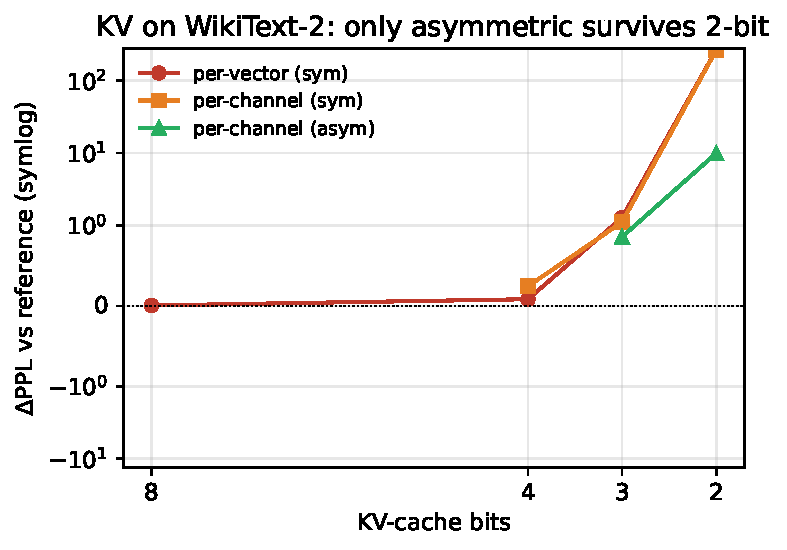
\includegraphics[width=\linewidth]{fig_kv_granularity.pdf}\end{minipage}
\hfill
\begin{minipage}{0.49\linewidth}\centering
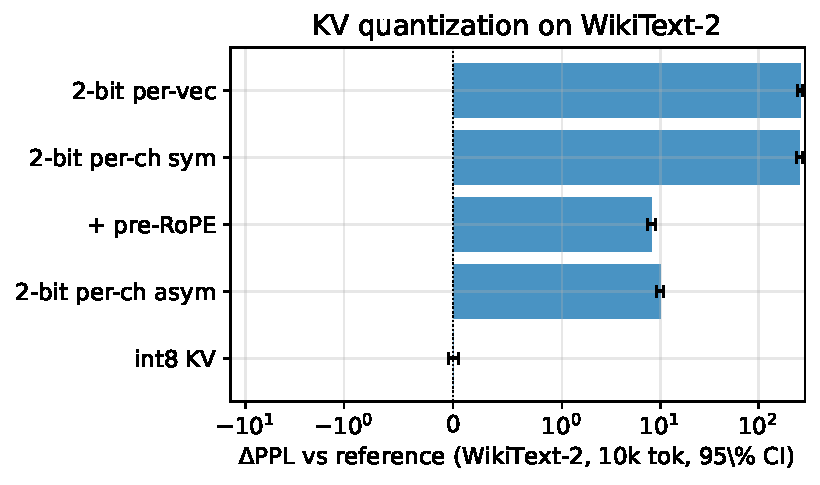
\includegraphics[width=\linewidth]{fig_kv_wikitext.pdf}\end{minipage}
\caption{KV-cache quantization, both panels on WikiText-2 (10{,}240 tokens). Left:
$\Delta$PPL vs bit-width by granularity (symlog). Right: the 2-bit configs with
bootstrap CIs. Per-vector \emph{and} per-channel-symmetric 2-bit both collapse
($+264$--$266$); only per-channel-\emph{asymmetric} keeps 2-bit nearly free ($+10$).
At this corpus size the zero-point, not granularity alone, sets the cliff.}
\label{fig:kv}
\end{figure}

\begin{table}[t]\centering\small
\caption{Integer-path KV-cache perplexity on WikiText-2 test (10{,}240 tokens). Int8
KV is free (CI spans 0); 2-bit \emph{per-vector and per-channel-symmetric both
collapse} ($+264$--$266$), and only the \emph{asymmetric} per-channel code rescues
2-bit ($+10$)---so at this corpus size granularity alone is not enough, the
zero-point is decisive. Robust activation scaling is catastrophic.}
\label{tab:wiki}
\begin{tabular}{lccc}
\toprule
Configuration & PPL & $\Delta$PPL & 95\% CI on $\Delta$PPL\\
\midrule
reference (absmax, KV float) & 27.4 & $+0.00$ & $[+0.00,\,+0.00]$\\
per-vector 8-bit & 27.4 & $+0.01$ & $[-0.04,\,+0.05]$\\
per-vector 2-bit (sym) & 293.2 & $+265.7$ & $[+247.9,\,+283.7]$\\
per-channel 2-bit (sym) & 291.5 & $+264.0$ & $[+246.2,\,+282.7]$\\
per-channel 2-bit (asym) & 37.4 & $\mathbf{+9.96}$ & $[+9.11,\,+10.87]$\\
\quad + pre-RoPE Keys & 35.6 & $+8.17$ & $[+7.43,\,+8.98]$\\
absmean activation scale & 1.7e5 & $+171080$ & $[+157977,\,+185339]$\\
\bottomrule
\end{tabular}
\\[2pt]{\footnotesize 10{,}240 tokens; paired token-level bootstrap, 2000 resamples.}
\end{table}


The ablation (Table~\ref{tab:ablation}) decomposes the 2-bit rescue. The
corpus-robust conclusion is that \emph{both} per-channel granularity \emph{and} a
zero-point are required: their combination (per-channel-asymmetric) is the only
config that holds at 2-bit on both corpora ($+0.9$ on the mini-corpus, $+10$ on
WikiText-2). Which single factor helps \emph{in isolation} is corpus-dependent and we
flag it rather than over-read it: on the mini-corpus per-channel-symmetric already
helps ($+11$) while per-vector-asymmetric hurts ($+175$, a zero-point wasting levels
when a vector spans an outlier); on the larger WikiText-2 set this reverses
(per-channel-symmetric collapses to $+264$, per-vector-asymmetric helps at $+125$).
The robust signal is the conjunction, not either marginal.

\begin{table}[t]\centering\small
\caption{2-bit KV-cache ablation, $\Delta$PPL on two corpora. The robust result is
the conjunction: only per-channel \emph{and} asymmetric holds on both. Which factor
helps \emph{alone} flips with corpus size---per-channel-symmetric helps on the
mini-corpus but collapses on WikiText-2; per-vector-asymmetric hurts on the
mini-corpus but helps on WikiText-2.}
\label{tab:ablation}
\begin{tabular}{lcc}
\toprule
2-bit KV configuration & mini-corpus (387 tok) & WikiText-2 (10k)\\
\midrule
per-vector, symmetric & $+86.9$ & $+265.7$\\
per-vector, asymmetric & $+175.1$ & $+124.6$\\
per-channel, symmetric & $+11.0$ & $+264.0$\\
per-channel, asymmetric & $\mathbf{+0.9}$ & $\mathbf{+10.0}$\\
\bottomrule
\end{tabular}
\\[2pt]{\footnotesize paired token-level bootstrap, 2000 resamples.}
\end{table}


\paragraph{Mechanism.} Figure~\ref{fig:mech}(left) measures the per-channel bias of
the Key and Value caches, $|\mu_c|/\sigma_c$. Key channels are off-center by
$\approx0.79\sigma$, $2.5\times$ the Value cache ($0.32\sigma$): a symmetric
quantizer, centered at zero, wastes about half its range on a biased channel, so a
per-channel zero-point recovers roughly a bit. This is the native-1-bit instance of
the Key-channel structure exploited by KIVI~\cite{liu2024kivi} and
KVQuant~\cite{hooper2024kvquant}; quantizing Keys pre-RoPE (Table~\ref{tab:wiki}) is
marginally better, consistent with RoPE mixing channels.

\begin{figure}[t]
\centering
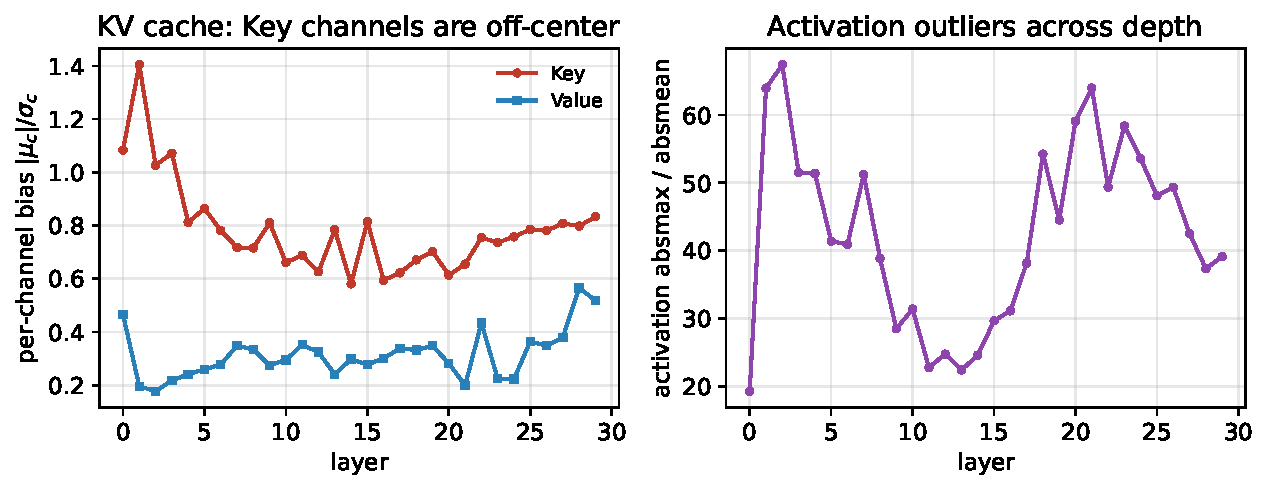
\includegraphics[width=0.92\linewidth]{fig_mechanism.pdf}
\caption{Mechanism. Left: per-channel bias $|\mu_c|/\sigma_c$ of Key vs Value across
layers---Keys are systematically off-center, explaining why asymmetric per-channel
KV recovers 2-bit. Right: activation absmax/absmean across layers (mean $42.6$),
the heavy tails behind the activation-scale fragility.}
\label{fig:mech}
\end{figure}

\section{Activation scaling is the load-bearing knob}
\label{sec:act}
The one component with no slack is the activation scale. Replacing absmax with
outlier-robust alternatives is catastrophic: on WikiText-2, absmean reaches
$1.7\times10^5$ perplexity (reference $27.4$). Figure~\ref{fig:rec} sweeps the
absmean clip multiplier: perplexity falls only as the multiplier grows past the
outliers---i.e.\ as the ``robust'' scale stops being robust. The cause is structural:
the activation absmax/absmean ratio has median $7.8$, p90 $\approx106$, max
$\approx1460$ (Figure~\ref{fig:mech}, right). In a quantization-aware-trained
W1.58A8 model the outliers \emph{are} the signal.

\begin{figure}[t]
\centering
\begin{minipage}{0.49\linewidth}\centering
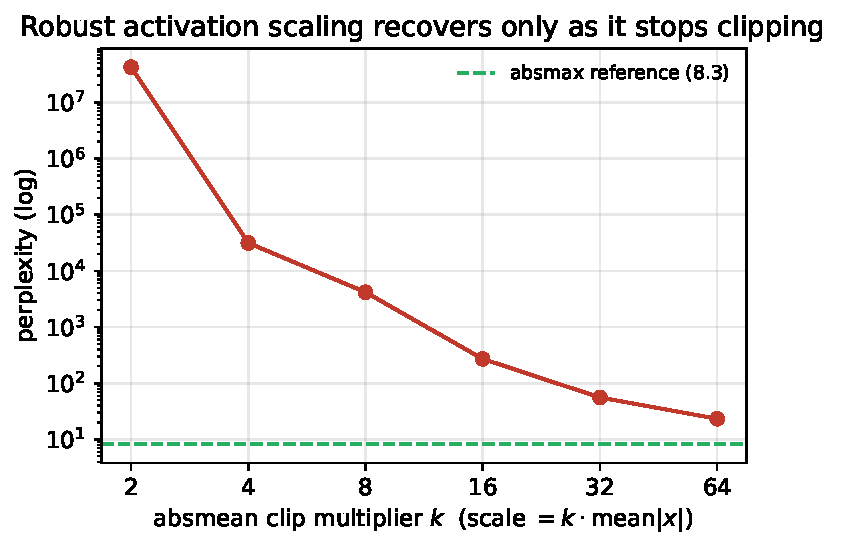
\includegraphics[width=\linewidth]{fig_act_recovery.pdf}\end{minipage}\hfill
\begin{minipage}{0.49\linewidth}\centering
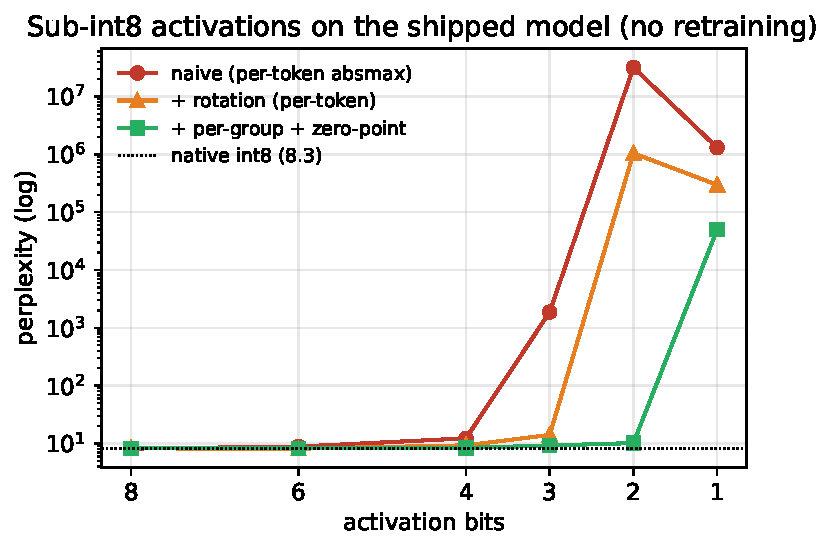
\includegraphics[width=\linewidth]{fig_actbits.pdf}\end{minipage}
\caption{Left: robust activation scaling recovers only as it stops clipping
outliers. Right: post-hoc activation quantization of the shipped model---naive
collapses below 8 bits; rotation reaches 4-bit; rotation + per-group scaling + a
2-bit zero-point (the KV cache's recipe) reaches \textbf{2-bit}, with 1-bit the floor
(Section~\ref{sec:rotate}).}
\label{fig:rec}
\end{figure}

\section{Preserve, don't suppress: the post-hoc activation frontier}
\label{sec:rotate}
Section~\ref{sec:act} and this one look contradictory: there, touching the
activation outliers is catastrophic; here, we transform them and low-bit
quantization becomes nearly free. The resolution is the central principle of this
paper, and it is sharper than ``outlier handling is the design axis'':
\textbf{outlier \emph{information} must be preserved; what is negotiable is only
whether it is concentrated or spread.} Robust (mean/median) scaling is
\emph{information-destroying}---it clips the outlier values and discards them. An
orthonormal rotation is \emph{information-preserving}---an invertible change of basis
that redistributes the same energy across coordinates without losing any. The two
results that appear to conflict are one law shown twice: one operation deletes the
signal, the other merely moves it.

This sharpens the novelty relative to QuaRot~\cite{ashkboos2024quarot}, which rotates
a full-precision model to remove outliers it treats as a \emph{nuisance}. Here
Section~\ref{sec:act} has just shown the outliers are load-bearing \emph{signal}, so
the a-priori prediction is that rotating them away destroys the model. It does
not---precisely because rotation preserves rather than suppresses---and that
non-obviousness is the contribution, not the port.

Concretely we quantize activations as $x\mapsto R^\top Q_b(Rx)$ with $R =
H_p\!\otimes\!O_m$ a normalized Sylvester Hadamard on the largest power-of-two factor
of the activation dimension and a fixed small orthogonal block on the remainder
($O(d\log d)$ cost); the ternary weights and the model are untouched and nothing is
retrained. Per-token rotation already recovers 4-bit activations ($+0.4$ PPL,
Table~\ref{tab:actbits}), reaching \emph{post-hoc} the int4-activation regime
BitNet~v2~\cite{wang2025bitnetv2} reached by \emph{retraining}. We are careful about
what this claims. A same-model head-to-head is not available: BitNet~v2 reports its
int4 results on separately retrained 1.3B/3B/7B models, and no int4-activation
weights are released for the 2B4T checkpoint we use, so there is no shared
(model, benchmark) pair to compare on. Both reach near-lossless int4 (theirs by
retraining, ours post-hoc at $+0.14$ PPL), but on different checkpoints; and the
usual PTQ-vs-QAT prior says retraining should still win at matched bits. We therefore
claim the same bit-width \emph{regime}, reached without retraining---not demonstrably
the same quality as a retrained model.

\paragraph{Granularity and a zero-point are the same lever for activations as for
the KV cache.} The KV-cache rescue (Section~\ref{sec:kv}) came from finer granularity
\emph{and} a zero-point; the identical pair applies here. Adding a per-group(32)
scale on top of the rotation extends the recovery to 3 bits ($+3.5\to\mathbf{+0.45}$
PPL on the short corpus, Table~\ref{tab:lowbit}); adding a per-group \emph{zero-point}
(asymmetric quantization) then reaches \textbf{2 bits}, where a symmetric code fails.
The decisive factor is exactly the one the KV cache flagged: a symmetric ``2-bit''
code wastes a level (it is effectively ternary), while an asymmetric 4-level code
uses all four. We report the magnitudes on a harder corpus and are explicit that the
int2 cost is corpus-dependent. On a WikiText-2 slice (512 tokens, reference $22.66$;
the $10{,}240$-token KV set of Table~\ref{tab:wiki} has reference $27.4$---same
configuration, longer slice, Table~\ref{tab:registry}): \textbf{int4} is free
($22.54$, $-0.1$), \textbf{int3} is $+2.1$, and \textbf{int2} (per-group(8)
asymmetric + rotation) is $\mathbf{+5.3}$ PPL---usable, and far below the
$+956$ of symmetric int2 or the $\sim\!10^6$ of naive int2 on the \emph{same} slice,
but a real cost, not the $+0.7$ the 133-token corpus suggested. So int2 activations
are reachable post-hoc by the asymmetric-granular recipe (the zero-point is the
load-bearing piece), at a corpus-dependent cost of roughly $1$--$5$ PPL.

\paragraph{Where post-hoc activation quantization stops: 1 bit.} To be explicit
about \emph{which} bit-width: this entire section varies the \emph{activation}
precision while the ternary 1.58-bit \emph{weights} are untouched (the model is
W1.58A8; ``1-bit'' in BitNet refers to weights, which we never change). For
activations, the post-hoc floor is one bit, not two: with only two levels, even
fine-group asymmetric quantization, rotation, and keeping the 128 largest channels
per token at int8 leaves 1-bit activations at $\sim\!2{\times}10^4$ PPL
($\sim\!4000\times$ the reference). This is the expected side of a well-known
asymmetry---static weights tolerate far lower bit-widths than dynamic, outlier-laden
activations, and sub-4-bit activations are known to require
QAT~\cite{wang2025bitnetv2}; we make no claim that 1-bit activations are unreachable
\emph{with} retraining, only that no post-hoc method we tried reaches them. The
honest post-hoc reach is \textbf{int8$\to$int2 activations} on the shipped model
(int4 free, int3 $\approx\!+2$ PPL, int2 $\approx\!+1$--$5$ PPL corpus-dependent),
with 1-bit the post-hoc floor---and 2-bit is reached by the \emph{same}
asymmetric-granular recipe the KV cache required.

\begin{table}[t]\centering\small
\caption{Sub-int8 activations on the shipped b1.58 (no retraining), perplexity
(native int8 reference $8.27$). Per-token rotation alone collapses below 4 bits;
the bottom row adds the KV-cache recipe (fine per-group scaling and, at 2 bits, a
zero-point), which reaches 2-bit. 1-bit is the floor.}
\label{tab:actbits}
\begin{tabular}{lcccccc}
\toprule
activation bits & 8 & 6 & 4 & 3 & 2 & 1\\
\midrule
naive (per-token absmax)     & $8.18$ & $8.86$ & $12.31$ & $1877$ & $3.2{\times}10^7$ & $1.3{\times}10^6$\\
\;+ rotation (per-token)     & $8.27$ & $8.15$ & $9.31$  & $14.09$& $1.0{\times}10^6$ & $3.0{\times}10^5$\\
\;+ per-group, +zero-point at 2b & --- & --- & $\mathbf{8.41}$ & $\mathbf{9.24}$ & $\mathbf{10.21}$ & $\sim\!5{\times}10^4$\\
\bottomrule
\end{tabular}
\\[2pt]{\footnotesize Bottom row: rotation + per-group(32) at 4/3-bit, + asymmetric
per-group(8) at 2-bit; native-int8 reference $8.27$. 1-bit resists every method.}
\end{table}

\begin{table}[t]\centering\small
\caption{The granularity\,+\,zero-point recipe, isolated (BitNet, short corpus, ref
$5.58$): $\Delta$PPL at 2-bit. Per-group scaling alone is not enough; the
\emph{zero-point} (asymmetric, 4-level vs.\ symmetric 3-level) is what makes 2-bit
work---the same factor that rescued the 2-bit KV cache. The mechanism holds on the
larger WikiText-2 slice: there per-group(8) asymmetric int2 is $+5.3$ PPL while
symmetric is $+956$ (Section~\ref{sec:rotate}); the asymmetric \emph{rescue} is
corpus-robust even though the absolute int2 cost grows on harder text.}
\label{tab:lowbit}
\begin{tabular}{lc}
\toprule
2-bit activation quantizer (with rotation) & $\Delta$PPL\\
\midrule
per-token, symmetric & $\sim\!10^6$\\
per-group(32), symmetric & $+1460$\\
per-group(16), \textbf{asymmetric} & $+1.4$\\
per-group(8), \textbf{asymmetric} & $\mathbf{+0.69}$\\
\bottomrule
\end{tabular}
\end{table}

\section{Cross-architecture generalization}
\label{sec:cross}
To test whether these are properties of one model or of native-1-bit inference,
we repeat the headline experiments on Falcon3-1B-1.58, an architecturally distinct
1-bit model (Llama-style: SwiGLU FFN, no sub-layer norms, an untied LM head, 18
layers, head dim 256), using the identical harness (the architecture profile is
auto-detected from the GGUF). Table~\ref{tab:crossmodel} reports $\Delta$PPL
\emph{on WikiText-2} (the same corpus as our main KV evidence, not the mini-corpus).
Every qualitative result transfers: int8 KV is free; at 2 bits per-vector \emph{and}
per-channel-symmetric KV both collapse ($+105$ and $+108$ for Falcon3) while only
per-channel-\emph{asymmetric} rescues it ($+18.5$); robust activation scaling is
catastrophic; and the mechanism is quantitatively the same---the Key per-channel bias
is $0.79\sigma$ in \emph{both} models. Two architectures at different scales (2B and
1B), built by different groups, exhibit the same integer-inference failure surface on
the same corpus, which is the evidence that this is about native-1-bit
\emph{quantization-aware training}, not a quirk of one checkpoint.

We flag the Key-bias coincidence rather than hide it: the per-channel bias matching
at $0.79\sigma$ to two significant figures across two architectures is more than our
$\sim\!1.5$k-token estimate resolves, so we read it as ``both clearly elevated and
near each other,'' not as a measured constant. We conjecture it is a genuine
attractor---absmax activation quantization plus RoPE applied to the Key projection
should induce a similar per-channel offset regardless of width or FFN type---but a
larger corpus and more models are needed to decide between ``invariant'' and
``coincidence.'' It is exactly the kind of striking regularity that should be stated
as a prediction (Section~\ref{sec:disc}), not oversold as a law.

\begin{table}[t]\centering\small
\caption{Cross-architecture generalization \emph{on WikiText-2} ($\Delta$PPL vs each
model's reference). The same failure surface holds across two architectures built by
different groups: int8 KV is free; 2-bit per-vector \emph{and} per-channel-symmetric
KV both collapse; only per-channel-\emph{asymmetric} rescues 2-bit; robust activation
scaling is catastrophic; and the Key per-channel bias is the same $0.79\sigma$ in
both. (BitNet on a 10k-token set, Falcon3-1B on a 1k-token set; see Table~\ref{tab:registry}.)}
\label{tab:crossmodel}
\begin{tabular}{lcc}
\toprule
& BitNet b1.58 2B4T & Falcon3-1B-1.58\\
2-bit KV / activation config & (ref $27.4$) & (ref $64.2$)\\
\midrule
int8 KV (per-vector) & $+0.01$ & $-0.27$\\
2-bit KV, per-vector & $+265.7$ & $+104.5$\\
2-bit KV, per-channel (sym) & $+264.0$ & $+107.7$\\
2-bit KV, per-channel (asym) & $\mathbf{+10.0}$ & $\mathbf{+18.5}$\\
absmean activation scale & $+1.7{\times}10^5$ & $+4.2{\times}10^3$\\
\midrule
Key per-channel bias $|\mu_c|/\sigma_c$ & $0.79$ & $0.79$\\
\bottomrule
\end{tabular}
\end{table}


\section{Discussion, implications, and predictions}
\label{sec:disc}
The integer-inference picture for this native-1-bit model inverts the usual
intuition. The fragile components are not the arithmetic primitives (integer
attention, fixed-point $\exp$, softmax normalization, KV bit-width to 3 bits) but
\emph{where the quantization grid sits and how fine it is}. The unifying law, stated
once: outlier \emph{information} must be preserved, and the only free variables are
how finely the grid is placed (granularity) and whether the basis concentrates or
spreads that information. Robust scaling loses; rotation and per-group/per-channel
granularity win---for the KV cache and for activations alike. To be precise about
``same lever'': granularity localizes the quantization grid in both cases, but the
\emph{outlier structure} it localizes against differs---the KV cache has per-channel
\emph{bias} (fixed by a zero-point), activations have heavy magnitude \emph{tails}
(fixed by a rotation). The shared principle is preserve-and-localize; the local
remedy is matched to the local structure.

\paragraph{Implications for edge inference (memory exactly; latency/energy expected).}
Every result is a lever for on-device deployment, where memory and bandwidth---not
FLOPs---bind. We quantify the memory effects, which are exact functions of the model
dimensions; latency and energy are \emph{expected} consequences we do not measure on
hardware here (Section~\ref{sec:limits}). (1) An integer-only datapath is achievable
end-to-end, including the rescale (integer multiply-shift), so no floating-point unit
is required, and a \emph{16-entry} $\exp$ LUT suffices for attention, so no precise
integer exponential is needed---both matter on microcontrollers and integer NPUs.
(2) KV cache: for BitNet 2B (30 layers, 5 KV heads, head dim 128) the cache is
$37.5$\,KB/token at int8, so a $4096$-token context costs $\approx\!150$\,MB;
per-channel-asymmetric \textbf{2-bit} KV cuts this to $9.4$\,KB/token and
$\approx\!38$\,MB ($4\times$) for $<10$ PPL---more on-device context per byte of
SRAM/DRAM. (3) Activations: a free $O(d\log d)$ rotation plus the same
fine-group asymmetric quantization reaches \textbf{int2} with no retraining
(Section~\ref{sec:rotate}), roughly a $4\times$ cut in activation memory and
bandwidth versus native int8. The headline: on the edge the
bits to cut are in the KV-cache and activations (via grid placement and granularity),
not in the softmax or attention precision.

\paragraph{Predictions (falsifiable, testable with our harness).} (1) The Key
per-channel bias, and thus the per-channel-asymmetric KV rescue, will appear in any
RoPE-based 1-bit model; (2) the activation absmax/absmean ratio predicts how badly
robust scaling fails and how few bits rotation buys; (3) applying the rotation
\emph{before} RoPE to Keys, and combining it with per-channel-asymmetric KV, will
compound (rotation reduces channel bias, asymmetry absorbs the residue). Our
single-model results are the first data point; the released harness is built to test
these across models and a full corpus.

\section{Hardware measurements (aarch64)}
\label{sec:hw}
BitNet's target is ARM CPUs, and on such hardware decoding is \emph{memory-bound}:
each token streams the weights and the KV cache, so bandwidth, not FLOPs, sets the
latency. We measure this directly with a small C microbenchmark on an aarch64 CPU
(NEON, int8 dot-product / i8mm) and report it in Table~\ref{tab:hw}. The sustained
read bandwidth is $47.5$\,GB/s; the 2-bit-packed ternary weights are $0.52$\,GB, so
the weight-streaming latency floor is $11$\,ms/token ($\approx\!90$ tok/s,
single-thread), in line with the $29$\,ms/token end-to-end that bitnet.cpp reports
for this model~\cite{ma2024bitnet2b4t}. The integer arithmetic is \emph{not} the
bottleneck (it hides under the memory stream with int8 SIMD), which is exactly why
an integer-only datapath is the right edge target. The KV-cache result is now
\emph{measured}, not inferred: at a 4096-token context the cache is $157$\,MB at int8
and $39$\,MB at 2-bit, and the corresponding per-token KV memory traffic falls from
$3.3$ to $0.8$\,ms---so the per-channel-asymmetric 2-bit KV cache of
Section~\ref{sec:kv} buys a $4\times$ reduction in both footprint and bandwidth on
real silicon. End-to-end, our pure-Rust port (Section~\ref{sec:repro}) decodes the
real model on an Apple-silicon laptop, and the two weight-storage choices expose the
memory--compute boundary directly (Table~\ref{tab:hw}, bottom). With weights
\emph{unpacked} to int8 it runs at $12.8$ tok/s but is \emph{memory-stalled}
(IPC $\approx\!1.0$, $4.2$\,GB). Storing them \emph{2-bit packed} cuts the footprint
to $2.7$\,GB as predicted, but decode drops to $6.1$ tok/s: it is now
\emph{compute-bound}, at IPC $\approx\!3.9$ while executing $8\times$ more
instructions to unpack the bits in scalar code. On this CPU the workload was not
actually bandwidth-bound ($\sim\!25$ of $\sim\!100$\,GB/s), so packing trades memory
stalls for unpacking compute.

\paragraph{The boundary condition (a prediction).} This is not a one-device anecdote
but an instance of a predictable threshold. Write decode time per token as a roofline
$t_{\text{unpacked}}=\max(W/B,\,M/C)$ and $t_{\text{packed}}=\max(W/4B,\,M/C+U)$,
where $W$ is the weight bytes streamed, $B$ memory bandwidth, $M/C$ the matmul compute
time, and $U$ the per-token unpack cost. Packing improves latency \emph{iff} the
device is weight-bandwidth-bound ($W/B$ is the binding term) \emph{and} the unpack
stays cheap enough, $U < W/B - W/4B = \tfrac{3}{4}\,W/B$. Our laptop sits on the wrong
side---compute-bound, so packing loses---while a bandwidth-starved target (a phone, or
a many-core part where $C$ is large and $B$ small) sits on the other, where packing
wins. The corollary is that a cheap unpack (small $U$, i.e.\ the SIMD shuffle kernel
bitnet.cpp uses---NEON unpacks 16 bytes to 64 ternary values in a few instructions)
moves the threshold so packing wins almost everywhere. Mapping this boundary across
devices ($B/C$ ratios), bit-widths, and unpack implementations is a natural and, we
think, sharper follow-up; here we locate it at one point and give the rule. (Both
artifacts are one command: \texttt{bench/kernels.c} and \texttt{cargo run}.)

\begin{table}[t]\centering\small
\caption{Hardware measurements, BitNet 2B. \emph{Top:} microbenchmark
(\texttt{bench/kernels.c}) on an aarch64 CPU---decoding is memory-bound, so the
2-bit weights/KV turn bandwidth into latency and footprint wins. \emph{Bottom:}
end-to-end decode of our pure-Rust port on an Apple-silicon laptop. The port stores
weights \emph{unpacked} (int8) for simplicity, so its footprint (4.2 GB) is $4\times$
the 0.52 GB a packed kernel would use; its throughput is single-core-scalar parallel
(no NEON), an honest floor.}
\label{tab:hw}
\begin{tabular}{lr}
\toprule
Quantity (4096 ctx) & Measured\\
\midrule
\multicolumn{2}{l}{\emph{microbenchmark (aarch64)}}\\
Sustained memory read bandwidth & $47.5$ GB/s\\
2-bit packed weights & $0.52$ GB\\
\;\;weight-stream latency floor & $11$ ms/token ($\approx\!90$ tok/s)\\
KV cache footprint, int8 $\to$ 2-bit & $157 \to 39$ MB ($4\times$)\\
KV memory traffic/token, int8 $\to$ 2-bit & $3.3 \to 0.8$ ms\\
\midrule
\multicolumn{2}{l}{\emph{end-to-end Rust port (Apple silicon), threaded}}\\
unpacked int8 weights & $12.8$ tok/s, $4.2$ GB\\
\;\;memory-stalled (IPC $\approx\!1.0$) & \\
2-bit packed weights & $6.1$ tok/s, $2.7$ GB\\
\;\;compute-bound unpack (IPC $\approx\!3.9$) & \\
\bottomrule
\end{tabular}
\end{table}

\section{Limitations}
\label{sec:limits}
We study two models (BitNet b1.58 2B4T and Falcon3-1B-1.58); the corpus is small
(a 387-token mini-corpus and a 10{,}240-token WikiText-2 set) to fit a CPU/numpy
reference, so absolute perplexities are not benchmark numbers, though the relative
effects and their CIs are stable across two corpora \emph{and} two architectures.
The KV/activation sweeps keep norm/RoPE/softmax in float (the fully-integer forms
are validated token-exact in Section~\ref{sec:cheap}, and the rescale is integer
multiply-shift), and the rotation study is post-training fake-quant. On the systems
side we measure memory bandwidth, weight/KV streaming latency, and an end-to-end
decode of the Rust port on Apple silicon (Section~\ref{sec:hw}); what we do
\emph{not} yet report is an \emph{optimized} engine---the port's scalar kernels are
either memory-stalled (unpacked, $12.8$ tok/s) or spend their cycles unpacking
(2-bit packed, $6.1$ tok/s), so both are floors, and an energy measurement is left to
future work. Closing the gap with a SIMD shuffle-unpack kernel (to get the packed
footprint at the unpacked speed) is engineering the characterization directly
motivates, not a change of method. The
remaining empirical breadth---full-corpus perplexity, the rotation result on the
larger slice, and a size ladder (Falcon3-3B/7B)---is a cheap extension with the
released one-command harness (\texttt{BN\_CORPUS}, \texttt{BITNET\_GGUF}), not a
change of method.

\section{Reproducibility}
\label{sec:repro}
We release a from-scratch reference (numpy oracle and integer engine), a pure-Rust
port with the \texttt{I2\_S} decoder checked bit-for-bit against Python, the
perplexity / bootstrap / mechanism / figure scripts, and the rotation study. Every
number here is produced by a script in the repository. Code, the per-token NLL
arrays backing every table and figure, and reproduction instructions are at
\url{https://github.com/kksante/bitnet-int8-rs} (commit \texttt{XXXXXXX}); model
weights are the public Microsoft and TII GGUF releases, not redistributed here.

\bibliographystyle{plain}
\begin{thebibliography}{99}
\bibitem{wang2023bitnet} H.~Wang et al. BitNet: Scaling 1-bit Transformers for Large
Language Models. arXiv:2310.11453, 2023.
\bibitem{ma2024era} S.~Ma et al. The Era of 1-bit LLMs: All Large Language Models are
in 1.58 Bits. arXiv:2402.17764, 2024.
\bibitem{ma2024bitnet2b4t} S.~Ma et al. BitNet b1.58 2B4T Technical Report.
arXiv:2504.12285, 2025.
\bibitem{wang2025bitnetcpp} J.~Wang et al. Bitnet.cpp: Efficient Edge Inference for
Ternary LLMs. arXiv:2502.11880, 2025.
\bibitem{wang2025bitnetv2} H.~Wang et al. BitNet v2: Native 4-bit Activations with
Hadamard Transformation for 1-bit LLMs. arXiv:2504.18415, 2025.
\bibitem{dettmers2022llmint8} T.~Dettmers et al. LLM.int8(): 8-bit Matrix
Multiplication for Transformers at Scale. NeurIPS, 2022.
\bibitem{xiao2023smoothquant} G.~Xiao et al. SmoothQuant: Accurate and Efficient
Post-Training Quantization for Large Language Models. ICML, 2023.
\bibitem{lin2023awq} J.~Lin et al. AWQ: Activation-aware Weight Quantization for LLM
Compression and Acceleration. arXiv:2306.00978, 2023.
\bibitem{ashkboos2024quarot} S.~Ashkboos et al. QuaRot: Outlier-Free 4-Bit Inference
in Rotated LLMs. NeurIPS, 2024.
\bibitem{li2026twla} Z.~Zhao et al. TWLA: Achieving Ternary Weights and Low-Bit
Activations for LLMs via Post-Training Quantization. ICML, 2026 (arXiv:2606.13054,
Jun.\ 2026; concurrent).
\bibitem{wang2026bwla} Z.~Zhao, Z.~Xu, D.~Yang. BWLA: Breaking the Barrier of W1AX
Post-Training Quantization for LLMs. arXiv:2605.00422, May 2026 (concurrent; same
group as~\cite{li2026twla}).
\bibitem{liu2024kivi} Z.~Liu et al. KIVI: A Tuning-Free Asymmetric 2bit Quantization
for KV Cache. ICML, 2024.
\bibitem{hooper2024kvquant} C.~Hooper et al. KVQuant: Towards 10 Million Context
Length LLM Inference with KV Cache Quantization. NeurIPS, 2024.
\bibitem{su2025rotatekv} Z.~Su et al. RotateKV: Accurate and Robust 2-Bit KV Cache
Quantization via Outlier-Aware Adaptive Rotations. arXiv:2501.16383, 2025.
\bibitem{merity2017wikitext} S.~Merity et al. Pointer Sentinel Mixture Models. ICLR,
2017.
\end{thebibliography}
\end{document}
